\documentclass{article}

% set font encoding for PDFLaTeX or XeLaTeX
\usepackage{ifxetex}
\ifxetex
  \usepackage{fontspec}
\else
  \usepackage[T1]{fontenc}
  \usepackage[utf8]{inputenc}
  \usepackage{lmodern}
    \usepackage{graphicx}
  \usepackage{float}
\fi

% used in maketitle
\title{Rotación(Sol-Tierra)}
\author{Eduardo Hndz\\Universidad De Sonora\\Lic. Física}

% Enable SageTeX to run SageMath code right inside this LaTeX file.
% documentation: http://mirrors.ctan.org/macros/latex/contrib/sagetex/sagetexpackage.pdf
% \usepackage{sagetex}

\begin{document}
\maketitle
\section{Introducción}
En esta actividad realizaremos la simulación de rotación de la tierra con respecto del sol.
Se nos pidió utilizar una función que nos calculara las coordenadas polares de dicha trayectoria, la cual aprendimos a usar y como observación la función va antes de iniciar el programa.

\subsection{código}
\begin{verbatim}
!introducimos una función que calcule X y Y en coordenadas polares
!o sea,X=rcos(theta) y Y=rsin(theta)
!donde r= 1.496d8 ya escrito en DP
!recuerda que estamos utilizando variables de doble precisión
!la función sehace antes del código del programa para llamarla después
!dentro de este

function funcx(theta) result(x)
    double precision, intent(in) ::theta
    double precision             ::x
    x=1.496d9*dcos(theta)
  end function funcx

  function funcy(theta) result(y)
    double precision, intent(in) ::theta
    double precision             :: y
    y=1.496d8*dsin(theta)
  end function funcy
!inciamos el programa
  program orbita
  implicit none
  !declaramos Constantes en DP
  !recuerda quela d(número) indicará la potencia a la que se
  !encuentra el número
  double precision, parameter:: pi=3.1416d0 
  !declaramos variables
  double precision::theta,funcy, funcx
  integer::i
  double precision,dimension(1000):: x, y
open(1, file= 'sol-tierra.dat' , status ='unknown')
  do i=1,360,1
     theta=dble(i)
     theta=(theta*pi)/180.0d0
     x(i)=funcx(theta)
     y(i)=funcy(theta)
     
     write(1,*) x(i), y(i)
     end do
     close(1)
end program orbita 
!
\end{verbatim}
El resultado de esta simulación fue como sigue
\begin{figure}[h!]
  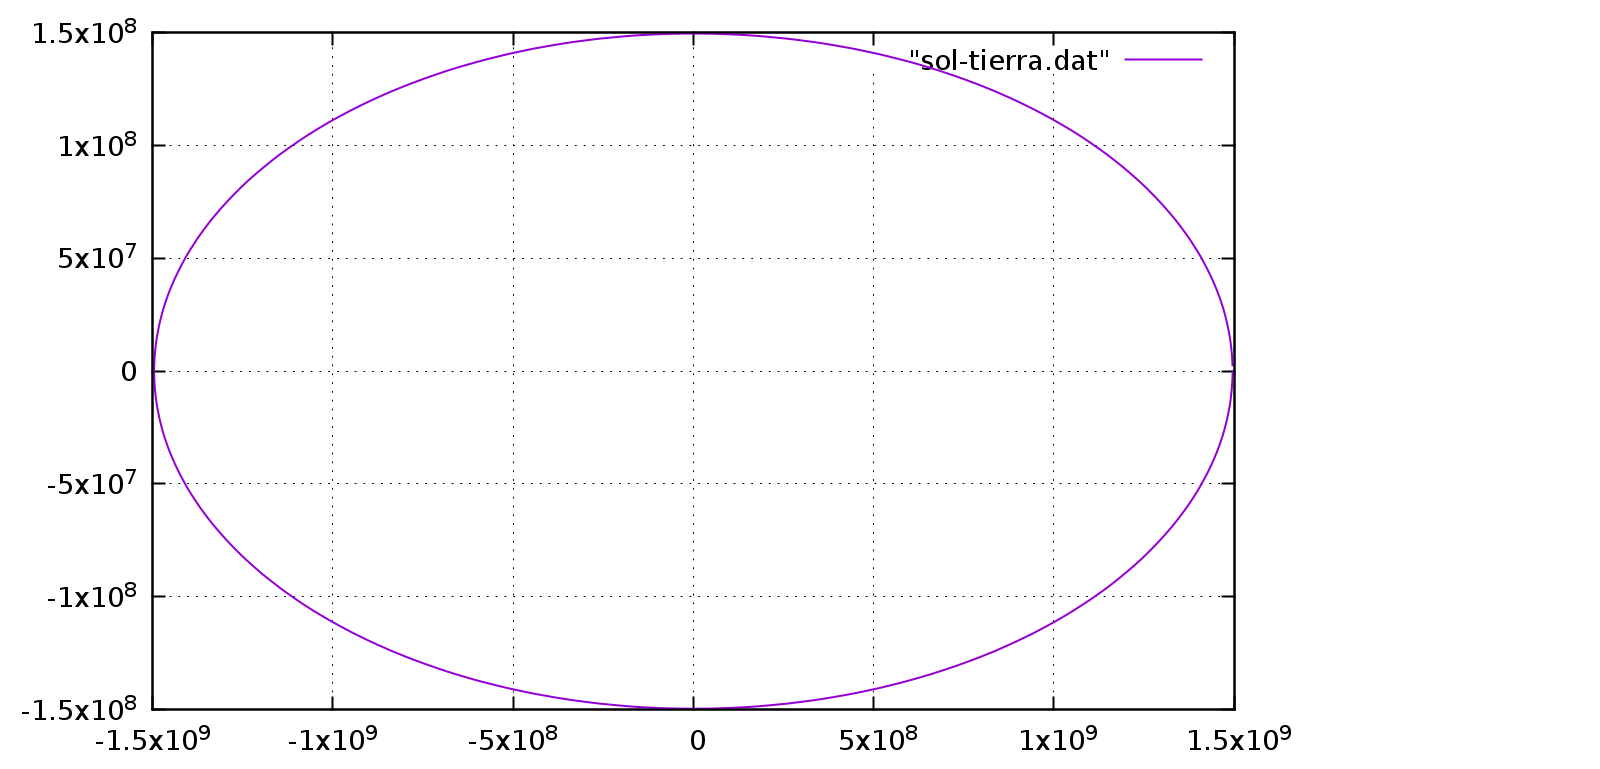
\includegraphics[width=\linewidth]{solt.png}
  \caption{final}
  \label{fig:boat1}
  \end{figure}
\end{document}
